\documentclass[9pt,aspectratio=169]{beamer}

% ============================================================
% PACKAGES
% ============================================================
\usepackage[utf8]{inputenc}
\usepackage[T1]{fontenc}
\usepackage{amsmath,amssymb}
\usepackage{graphicx}
\graphicspath{{result images/}{}}
\usepackage{xcolor}
\usepackage{booktabs}
\usepackage{multirow}
\usepackage{array}
\usepackage{hyperref}
\usepackage{lmodern}
\usepackage{tikz}
\usetikzlibrary{positioning,arrows.meta,calc}

% ============================================================
% THEME
% ============================================================
\usetheme{Madrid}
\usecolortheme{seahorse}
\setbeamertemplate{navigation symbols}{}
\setbeamertemplate{footline}{%
  \leavevmode%
  \hbox{%
    \begin{beamercolorbox}[wd=.5\paperwidth,ht=2.25ex,dp=1ex,left,leftskip=1em]{author in head/foot}%
      \usebeamerfont{author in head/foot}\insertshortauthor\ |\ \insertshortinstitute
    \end{beamercolorbox}%
    \begin{beamercolorbox}[wd=.4\paperwidth,ht=2.25ex,dp=1ex,center]{title in head/foot}%
      \usebeamerfont{title in head/foot}\insertshorttitle
    \end{beamercolorbox}%
    \begin{beamercolorbox}[wd=.1\paperwidth,ht=2.25ex,dp=1ex,right,rightskip=1em]{date in head/foot}%
      \usebeamerfont{date in head/foot}\insertframenumber/\inserttotalframenumber
    \end{beamercolorbox}}%
}
\setbeamerfont{frametitle}{size=\small,series=\bfseries}
\setbeamerfont{title}{size=\large,series=\bfseries}
\setbeamerfont{subtitle}{size=\footnotesize}
\setbeamerfont{block title}{size=\footnotesize,series=\bfseries}
\setbeamerfont{block body}{size=\footnotesize}
\setbeamertemplate{itemize items}[circle]
\setbeamertemplate{enumerate items}[default]

% Tighten list spacing globally
\setlength{\leftmargini}{1.1em}
\setlength{\leftmarginii}{0.9em}
\setlength{\itemsep}{0pt}
\setlength{\parskip}{0pt}

% ============================================================
% COLOURS
% ============================================================
\definecolor{darkred}{RGB}{150,20,20}
\definecolor{steelblue}{RGB}{50,90,160}
\definecolor{forestgreen}{RGB}{30,110,50}

% ============================================================
% TITLE PAGE
% ============================================================
\title[Schema Unification for Credit Risk]{%
  Schema Unification for Credit Risk:\\[2pt]
  An Empirical Study of Dataset Aggregation}

\subtitle{Universal Credit Risk Schema (UCRS) · XGBoost · Cross-Dataset Evaluation}

\author[Jain \& Goswami]{%
  Ravi Kumar Jain\textsuperscript{1} \quad Dr.\ Anju Goswami\textsuperscript{2}}

\institute[IIFT New Delhi]{%
  \textsuperscript{1,2}Indian Institute of Foreign Trade (IIFT), New Delhi, India\\[4pt]
  \texttt{ravi\_phdm23@iift.edu} \quad|\quad \texttt{anju@iift.edu}}

\date{}

% ============================================================
\begin{document}
% ============================================================

% SLIDE 1 — TITLE
\begin{frame}
  \titlepage
\end{frame}

% SLIDE 2 — OUTLINE
\begin{frame}{Outline}
  \tableofcontents
\end{frame}

% ===========================================================
\section{Motivation \& Research Gap}
% ===========================================================

% SLIDE 3 — MOTIVATION
\begin{frame}{Motivation}
\vspace{-2pt}
\begin{block}{Context}
  \footnotesize
  Doctoral research in credit risk prediction works with multiple public datasets
  --- each using different independent variables to describe the same borrower
  behaviour.\\[2pt]
  The question that follows: is there a right, common set of independent variables
  that can represent all these sources --- and support a single unified model?
\end{block}
\vspace{4pt}
\begin{columns}[T]
  \column{0.55\textwidth}
    \textbf{The Research Question}
    \begin{itemize}\setlength\itemsep{3pt}
      \item[\small$\bullet$] Multiple public credit datasets exist — each with different
            variable names, formats, and definitions
      \item[\small$\bullet$] Can a \textbf{single model}, trained on all of them together,
            serve predictions across every source — without retraining per dataset?
      \item[\small$\bullet$] Common variables (e.g., age, income) appear across sources —
            will \textbf{pooled learning improve their predictive signal}, especially
            for small datasets?
      \item[\small$\bullet$] \textbf{Prerequisite:} variables must first be harmonised into
            a common schema before any joint training is possible
    \end{itemize}

  \column{0.42\textwidth}
    \begin{block}{Potential Applications}
      \footnotesize
      \begin{itemize}\setlength\itemsep{2pt}
        \item Multiple institutions in a region hold small, isolated credit
              datasets with overlapping attributes
        \item A standardised schema could enable pooling across institutions
              — training one shared model
        \item A new entrant institution could leverage this pre-trained model
              without requiring its own historical data
      \end{itemize}
    \end{block}
    \vspace{4pt}
    \begin{alertblock}{Research Gap}
      \footnotesize
      No prior work has applied a \textbf{standardised schema} (e.g., the Five Cs) to
      \emph{aggregate} heterogeneous credit datasets for joint training and
      rigorous cross-dataset evaluation.
    \end{alertblock}
\end{columns}
\end{frame}

% ===========================================================
\section{Research Objectives}
% ===========================================================

% SLIDE 4 — RESEARCH OBJECTIVES
\begin{frame}{Research Objectives}
\vspace{8pt}
\begin{enumerate}\setlength\itemsep{10pt}
  \item Test the hypothesis that aggregating multiple heterogeneous credit
        datasets into a single unified dataset improves predictive performance
        --- demonstrated using four publicly available credit datasets as the
        empirical test case

  \item Develop a \textbf{Universal Credit Risk Schema (UCRS)} --- a common
        set of canonical variables ensuring that the same concept carries the
        same name and meaning regardless of the source dataset

  \item Standardise \textbf{categorical variable values} across datasets so
        that the same category carries the same meaning --- for example,
        marital status or employment type coded differently across sources

  \item \textbf{Validate} the concept by training an XGBoost model on the
        unified dataset and comparing its performance against models trained
        individually on each source dataset
\end{enumerate}
\end{frame}

% ===========================================================

% ===========================================================
\section{Literature Review}
% ===========================================================

% SLIDE A -- LITERATURE REVIEW (I): FOUNDATIONS
\begin{frame}{Literature Review (I): Theoretical Foundations}
\vspace{-4pt}
\begin{columns}[T]
  \column{0.48\textwidth}
    \begin{block}{1.\ Data Harmonisation \& Integration}
      \footnotesize
      \begin{itemize}\setlength\itemsep{2pt}
        \item Cheng et al.\ (2024) --- schema alignment is required before
              any cross-dataset analysis can be conducted
        \item Asthana \& Mahindru (2022) --- financial datasets lack
              consistent variable definitions across institutions
      \end{itemize}
    \end{block}
    \vspace{5pt}
    \begin{block}{2.\ Heterogeneous Data \& Features}
      \footnotesize
      \begin{itemize}\setlength\itemsep{2pt}
        \item Hayashi \& Takano (2020) --- identical variable names across
              sources do not guarantee conceptual equivalence; careful
              feature alignment is essential
      \end{itemize}
    \end{block}

  \column{0.48\textwidth}
    \begin{block}{3.\ Conceptual Foundations}
      \footnotesize
      \begin{itemize}\setlength\itemsep{2pt}
        \item Hand \& Henley (1997); Thomas (2000) --- credit scoring as
              statistical classification; foundational definitions
        \item Baesens et al.\ (2003) --- algorithm benchmarking in credit risk
        \item Baiden (2011) --- defines the Five Cs framework as the core
              tool for credit underwriting decisions
        \item Marqu\'{e}s et al.\ (2013) --- bridges the Five Cs to modern
              ML-based credit scoring; grounds UCRS schema design
      \end{itemize}
    \end{block}
    \vspace{5pt}
    \begin{block}{4.\ Dataset Aggregation \& Transfer Learning}
      \footnotesize
      \begin{itemize}\setlength\itemsep{2pt}
        \item Ni et al.\ (2022) --- multi-source enrichment for corporate credit
        \item Zhang et al.\ (2025) --- cross-domain credit via domain adaptation
        \item Pan \& Yang (2010); Ben-David et al.\ (2010) --- theoretical basis
              for learning across different distributions
      \end{itemize}
    \end{block}
\end{columns}
\end{frame}

% SLIDE B -- LITERATURE REVIEW (II): METHODOLOGY
\begin{frame}{Literature Review (II): Methodology Support}
\vspace{-4pt}
\begin{columns}[T]
  \column{0.48\textwidth}
    \begin{block}{5.\ Credit Risk ML --- Algorithm Selection}
      \footnotesize
      \begin{itemize}\setlength\itemsep{2pt}
        \item Lessmann et al.\ (2015) --- 41 classifiers benchmarked;
              ensemble methods consistently top performers
        \item Chen \& Guestrin (2016) --- XGBoost: scalable tree boosting
        \item Xia et al.\ (2024); Chen et al.\ (2024) --- XGBoost for
              large-scale credit datasets
        \item Akinjole et al.\ (2024); Li et al.\ (2021) --- ensemble
              methods with resampling for credit default
      \end{itemize}
    \end{block}
    \vspace{5pt}
    \begin{block}{6.\ Ensemble Theory \& Interpretability}
      \footnotesize
      \begin{itemize}\setlength\itemsep{2pt}
        \item Friedman (2001); Breiman (1996) --- gradient boosting and
              bagging: theoretical foundations
        \item Sagi \& Rokach (2018) --- ensemble learning survey
        \item Lundberg \& Lee (2017) --- SHAP: a unified approach to
              post-hoc model interpretability
      \end{itemize}
    \end{block}

  \column{0.48\textwidth}
    \begin{block}{7.\ Class Imbalance \& Data Quality}
      \footnotesize
      \begin{itemize}\setlength\itemsep{2pt}
        \item Chawla et al.\ (2002) --- SMOTE: synthetic minority
              oversampling to address class imbalance
        \item He \& Garcia (2009) --- learning from imbalanced data
        \item Louzada et al.\ (2016) --- binary classification methods
              in credit scoring: a systematic review
      \end{itemize}
    \end{block}
    \vspace{5pt}
    \begin{alertblock}{Collective Research Gap}
      \footnotesize
      Each strand of literature addresses one challenge in isolation.
      No prior work combines schema harmonisation, multi-source
      aggregation, and empirical validation into a single unified
      credit risk modelling framework.
    \end{alertblock}
\end{columns}
\end{frame}

% ===========================================================
\section{Methodology}
% ===========================================================

% SLIDE 7 — DATA SOURCES
\begin{frame}{Data Sources}
\vspace{-2pt}
{\footnotesize Four publicly available datasets sourced from distinct geographical and institutional contexts ---
spanning small-scale benchmark datasets to large-scale competition data.}\\[5pt]
\begin{center}
\scriptsize
\setlength{\tabcolsep}{4pt}
\begin{tabular}{l l r r l p{5.2cm}}
  \toprule
  \textbf{Dataset} & \textbf{Credit Market} & \textbf{Records} & \textbf{Feat.} & \textbf{Source} & \textbf{Key Characteristic}\\
  \midrule
  German Credit  & Consumer credit (Germany) &  1,400 & 20 & UCI Statlog   & Classical benchmark; widely used for algorithm benchmarking; mixed ordered categorical variables\\[3pt]
  HELOC          & Home equity (US)          & 10,918 & 23 & FICO / Kaggle & Credit bureau data; features include delinquency counts, utilisation ratios, and revolving credit metrics\\[3pt]
  Taiwan UCI     & Credit card (Taiwan)      & 46,728 & 23 & UCI           & Rich temporal payment history --- PAY\_0 to PAY\_6 captures six months of lagged payment behaviour\\[3pt]
  PAK (PAKDD 09) & P2P lending               & 73,918 & 25 & PAKDD 2009    & Competition data with realistic income filters; cost-sensitive, imbalanced default scenarios\\[3pt]
  \midrule
  \textbf{Combined (UCRS)} & \textbf{All four markets} & \textbf{132,964} & \textbf{107} & \textbf{UCRS} & \textbf{Unified under Five Cs schema}\\
  \bottomrule
\end{tabular}
\end{center}
\vspace{4pt}
\begin{block}{Why these four datasets?}
  \footnotesize
  All four are publicly available, carry a clear binary default label, and represent heterogeneous
  borrower populations, risk horizons, and data collection practices --- making them well-suited
  for testing whether a single unified model can generalise across diverse credit contexts.
\end{block}
\end{frame}

% SLIDE 8 — UCRS SCHEMA
\begin{frame}{Universal Credit Risk Schema (UCRS)}
\vspace{-2pt}
\begin{center}
\footnotesize
\begin{tabular}{p{1.6cm} p{4.2cm} p{5.8cm}}
  \toprule
  \textbf{Five C} & \textbf{Credit Rationale} & \textbf{Variable Coverage}\\
  \midrule
  Character   & Historical repayment willingness        & Demographics, employment history, credit score\\
  Capacity    & Cash-flow headroom for new debt         & Income, loan amount, DTI ratio, savings accounts\\
  Capital     & Financial cushion against income shocks & Property ownership, net worth, dependents, assets\\
  Collateral  & Lender's recovery position              & Collateral type, co-borrowers, guarantor, residence\\
  Conditions  & Dynamic credit-bureau signals           & 6-month payment history, utilisation, delinquency, trade counts\\
  \midrule
  \textbf{Total (UCRS)} & \multicolumn{2}{l}{\textbf{Unified canonical feature space grounded in the Five Cs of credit}}\\
  \bottomrule
\end{tabular}\\[3pt]
{\scriptsize\textit{Five Cs framework adopted from: Baiden, J.\ E.\ (2011). The 5 C's of credit. \textit{SSRN Electronic Journal}; Marqu\'{e}s et al.\ (2013). \textit{Expert Systems with Applications}, 39(12).}}
\end{center}
\vspace{4pt}
{\footnotesize Each source dataset uses different variable names for the same concept.
The alias mapping resolves these to a single canonical UCRS name before training.}\\[4pt]
\begin{center}
\footnotesize\textbf{Alias mapping --- sample (Capacity dimensions)}\\[3pt]
\begin{tabular}{llll}
  \toprule
  \textbf{UCRS Canonical Variable} & \textbf{PAK} & \textbf{Taiwan UCI} & \textbf{HELOC}\\
  \midrule
  \texttt{LOAN\_AMOUNT}     & loan\_amount     & LIMIT\_BAL  & credit\_limit\\
  \texttt{MONTHLY\_INCOME}  & monthly\_income  & (account)   & income\\
  \texttt{DEBT\_TO\_INCOME} & debt\_to\_income & (payment)   & dti\_ratio\\
  \bottomrule
\end{tabular}
\end{center}
\end{frame}

% ===========================================================
% SLIDE 9 — UCRS MAPPING MATRIX — UNIFIED STRUCTURE & COVERAGE
% ===========================================================
\begin{frame}{UCRS Attribute Mapping: Structure \& Dataset Coverage}
\vspace{-4pt}
\begin{center}
\footnotesize
\setlength{\tabcolsep}{4pt}
\begin{tabular}{llcc|cccc}
\toprule
\textbf{Five C} & \textbf{Sub-group} & \textbf{Dims} & \textbf{Representative Variables} & \textbf{PAK} & \textbf{Taiwan} & \textbf{German} & \textbf{HELOC}\\
\midrule
\multirow{4}{*}{\textbf{Character (21)}}
  & Demographics  &  5 & Age, Gender, Marital Status         & \multirow{4}{*}{14} & \multirow{4}{*}{4}  & \multirow{4}{*}{8} & \multirow{4}{*}{---}\\
  & Employment    &  8 & Tenure, Sector, Status              & & & & \\
  & Credit Hist.  &  4 & Credit Score, Bureau Record         & & & & \\
  & Verification  &  4 & Income Proof, Phone, Email          & & & & \\
\cmidrule{1-8}
\multirow{3}{*}{\textbf{Capacity (19)}}
  & Income \& Debt &  6 & Salary, DTI Ratio, Dependents      & \multirow{3}{*}{3}  & \multirow{3}{*}{1}  & \multirow{3}{*}{7} & \multirow{3}{*}{---}\\
  & Loan Details   &  7 & Amount, Purpose, Tenure            & & & & \\
  & Accounts       &  6 & Checking, Savings, Credit Cards    & & & & \\
\cmidrule{1-8}
\multirow{2}{*}{\textbf{Capital (11)}}
  & Assets    &  6 & Property, Vehicles, Net Worth           & \multirow{2}{*}{5}  & \multirow{2}{*}{---} & \multirow{2}{*}{3} & \multirow{2}{*}{---}\\
  & Financial &  5 & Housing Status, Savings                 & & & & \\
\cmidrule{1-8}
\textbf{Collateral (5)} & Security & 5 & Type, Co-borrower, Guarantor      & 1  & --- & 2  & ---\\
\cmidrule{1-8}
\multirow{3}{*}{\textbf{Conditions (51)}}
  & Payment History & 20 & Payment Status, Bill \& Pay Amounts & \multirow{3}{*}{1}  & \multirow{3}{*}{19} & \multirow{3}{*}{2} & \multirow{3}{*}{14}\\
  & Bureau Signals  & 18 & Trade Counts, Utilisation Ratios    & & & & \\
  & Behavioural     & 13 & Inquiries, Account Age, Delinquency & & & & \\
\midrule
\textbf{Total} & & \textbf{107} & & \textbf{24} & \textbf{24} & \textbf{22} & \textbf{14}\\
\bottomrule
\end{tabular}
\end{center}
\vspace{2pt}
{\scriptsize\textit{Dataset columns show attributes mapped per Five-C category. UCRS unifies all 107 dimensions into a single canonical feature space grounded in the Five Cs of credit.}}
\end{frame}

% SLIDE 10 — EXPERIMENTAL PIPELINE
\begin{frame}{Experimental Pipeline}
\vspace{-4pt}
\begin{columns}[T]
  \column{0.55\textwidth}
    \vspace{-2pt}
    \begin{center}
    \resizebox{\linewidth}{!}{%
    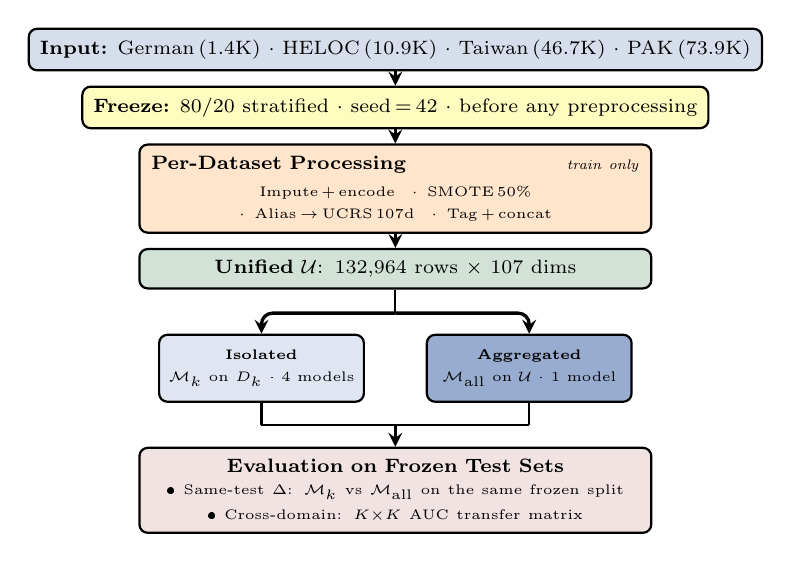
\begin{tikzpicture}[
        mbox/.style={draw, rounded corners=3pt, align=center, minimum width=6.5cm,
                     inner sep=4pt, font=\scriptsize, thick},
        tbox/.style={draw, rounded corners=3pt, align=center, minimum width=2.6cm,
                     minimum height=0.85cm, inner sep=3pt, font=\tiny, thick},
        arr/.style={->, very thick, >=stealth}
    ]
    \node[mbox, fill=steelblue!20] (inp) at (0,0) {%
      \textbf{Input:} German\,(1.4K) $\cdot$ HELOC\,(10.9K) $\cdot$ Taiwan\,(46.7K) $\cdot$ PAK\,(73.9K)%
    };
    \node[mbox, fill=yellow!25, below=0.18cm of inp] (spl) {%
      \textbf{Freeze:} 80/20 stratified $\cdot$ seed\,=\,42 $\cdot$ before any preprocessing%
    };
    \node[mbox, fill=orange!20, text width=6.2cm, below=0.18cm of spl] (prc) {%
      \textbf{Per-Dataset Processing} \hfill \textit{\tiny train only}\\[2pt]
      \tiny Impute\,+\,encode \enspace$\cdot$\enspace SMOTE\,50\% \enspace$\cdot$\enspace Alias$\,\to\,$UCRS\,107d \enspace$\cdot$\enspace Tag\,+\,concat%
    };
    \node[mbox, fill=forestgreen!20, below=0.18cm of prc] (uni) {%
      \textbf{Unified} $\mathcal{U}$:\enspace 132{,}964 rows $\times$ 107 dims%
    };
    \node[tbox, fill=steelblue!15] (iso) at ($(uni.south)+(-1.7,-1.00)$) {%
      \textbf{Isolated}\\[2pt]$\mathcal{M}_k$ on $D_k$ · 4 models%
    };
    \node[tbox, fill=steelblue!50] (agg) at ($(uni.south)+(+1.7,-1.00)$) {%
      \textbf{Aggregated}\\[2pt]$\mathcal{M}_{\text{all}}$ on $\mathcal{U}$ · 1 model%
    };
    \node[mbox, fill=darkred!12, text width=6.2cm] (evl) at ($(uni.south)+(0,-2.55)$) {%
      \textbf{Evaluation on Frozen Test Sets}\\[2pt]
      \tiny\textbullet\ Same-test $\Delta$: $\mathcal{M}_k$ vs $\mathcal{M}_{\text{all}}$ on the same frozen split\\[1pt]
      \tiny\textbullet\ Cross-domain: $K{\times}K$ AUC transfer matrix%
    };
    \draw[arr] (inp) -- (spl);
    \draw[arr] (spl) -- (prc);
    \draw[arr] (prc) -- (uni);
    \coordinate (fk) at ($(uni.south)+(0,-0.30)$);
    \draw[thick] (uni.south) -- (fk);
    \draw[arr, rounded corners=4pt] (fk) -- +(-1.7,0) -- (iso.north);
    \draw[arr, rounded corners=4pt] (fk) -- +(+1.7,0) -- (agg.north);
    \coordinate (jl) at ($(iso.south)+(0,-0.28)$);
    \coordinate (jr) at ($(agg.south)+(0,-0.28)$);
    \coordinate (jm) at ($(jl)!0.5!(jr)$);
    \draw[thick] (iso.south) -- (jl);
    \draw[thick] (jl) -- (jr);
    \draw[thick] (agg.south) -- (jr);
    \draw[arr] (jm) -- (evl.north);
    \end{tikzpicture}%
    }
    \end{center}

  \column{0.42\textwidth}
    \footnotesize\textbf{Two Training Regimes}
    \begin{enumerate}\setlength\itemsep{3pt}
      \item \textbf{Isolated} — XGBoost trained separately on each dataset; establishes per-source baseline (4 models)
      \item \textbf{Aggregated} — single XGBoost trained on the full unified UCRS dataset (1 model)
    \end{enumerate}
    \vspace{5pt}
    \footnotesize\textbf{Evaluation Metrics}
    \begin{itemize}\setlength\itemsep{4pt}
      \item[\small$\bullet$] \textbf{AUC-ROC} — primary metric; measures discriminative power across all classification thresholds; robust to class imbalance
      \item[\small$\bullet$] \textbf{PR-AUC} — precision-recall performance; informative when positive class is rare
      \item[\small$\bullet$] \textbf{Accuracy \& Balanced Accuracy} — overall correctness and class-adjusted correctness
      \item[\small$\bullet$] \textbf{F1 Score} — harmonic mean of precision and recall
      \item[\small$\bullet$] \textbf{Specificity \& Recall} — reported in confusion matrix analysis
    \end{itemize}
\end{columns}
\end{frame}

% ===========================================================
\section{Results}
% ===========================================================

% SLIDE 11 — OVERALL PERFORMANCE
\begin{frame}{Overall Predictive Performance}
\vspace{-2pt}
\begin{columns}[T]
  \column{0.62\textwidth}
    \begin{tikzpicture}
      \node[anchor=north west, inner sep=0pt] (chart) at (0,0) {%
        \includegraphics[width=\linewidth,height=0.52\textheight,keepaspectratio]{metric_comparison.png}%
      };
      \draw[steelblue, line width=1.8pt, rounded corners=3pt]
        let \p1 = ($(chart.west)!0.785!(chart.east)$),
            \p2 = ($(chart.west)!0.995!(chart.east)$),
            \p3 = ($(chart.south)!0.88!(chart.north)$),
            \p4 = ($(chart.south)!0.09!(chart.north)$)
        in (\x1,\y3) rectangle (\x2,\y4);
    \end{tikzpicture}
    \vspace{3pt}
    \scriptsize
    \setlength{\tabcolsep}{4pt}
    \begin{tabular}{lrrr}
      \toprule
      \textbf{Dataset} & \textbf{Rows} & \textbf{Features} & \textbf{UCRS Mapped}\\
      \midrule
      German Credit &  1,400 & 20 & 22\\
      HELOC         & 10,918 & 23 & 14\\
      Taiwan UCI    & 46,728 & 23 & 24\\
      PAK           & 73,918 & 25 & 24\\
      \bottomrule
    \end{tabular}

  \column{0.35\textwidth}
    \begin{itemize}\setlength\itemsep{4pt}
      \item[\small$\bullet$] \textbf{Taiwan UCI} achieves the strongest individual AUC (0.884)
      \item[\small$\bullet$] Combined model occupies an \textbf{intermediate band} — above German Credit and HELOC, below Taiwan UCI
      \item[\small$\bullet$] Expected: pooled model optimises across \emph{heterogeneous} distributions simultaneously
    \end{itemize}
    \vspace{5pt}
    \begin{block}{Key observation}
      \footnotesize
      The combined UCRS model performs within the range of individually
      trained models --- competitive across all four datasets without
      being trained exclusively on any single one.
    \end{block}
\end{columns}
\end{frame}

% SLIDE 12 — ROC & PR CURVES
\begin{frame}{ROC and Precision-Recall Curves}
\vspace{-4pt}
\begin{columns}[T]
  \column{0.50\textwidth}
    \begin{center}
      \footnotesize\textbf{ROC Curves by Dataset}\\[2pt]
      \includegraphics[width=\linewidth,height=0.54\textheight,keepaspectratio]{roc_curves.png}
    \end{center}
  \column{0.48\textwidth}
    \begin{center}
      \footnotesize\textbf{Precision-Recall Curves by Dataset}\\[2pt]
      \includegraphics[width=\linewidth,height=0.54\textheight,keepaspectratio]{precision_recall_curves.png}
    \end{center}
\end{columns}
\vspace{4pt}
\begin{columns}[T]
  \column{0.48\textwidth}
    \footnotesize\textbf{What these metrics measure}
    \begin{itemize}\setlength\itemsep{2pt}
      \item[\small$\bullet$] \textbf{AUC-ROC} — how well the model separates defaulters from non-defaulters across all decision thresholds; 0.5 = random, 1.0 = perfect
      \item[\small$\bullet$] \textbf{PR-AUC} — precision-recall balance when defaulters are rare; more sensitive to class imbalance than AUC-ROC
    \end{itemize}
  \column{0.48\textwidth}
    \footnotesize\textbf{Observations}
    \begin{itemize}\setlength\itemsep{2pt}
      \item[\small$\bullet$] \textbf{Taiwan UCI} leads on both curves — AUC 0.884, PR-AUC 0.918
      \item[\small$\bullet$] \textbf{Combined UCRS model} (red) maintains consistently strong curves across all four datasets
      \item[\small$\bullet$] \textbf{HELOC} shows the weakest PR curve — limited discriminative signal in its feature set
    \end{itemize}
\end{columns}
\end{frame}

% SLIDE 9 — SAME-TEST COMPARISON
\begin{frame}{Does Aggregation Improve Performance?}
\vspace{-2pt}
\begin{columns}[T]
  \column{0.55\textwidth}
    \begin{center}
      \includegraphics[width=\linewidth,height=0.73\textheight,keepaspectratio]{combined_delta_metrics.png}
    \end{center}

  \column{0.42\textwidth}
    \textcolor{forestgreen}{\textbf{Gains from pooling}}
    \begin{itemize}\setlength\itemsep{3pt}
      \item[\small$\bullet$] \textbf{German Credit} (+0.016 AUC): only 1,120 training rows — pooled corpus adds richer signal
      \item[\small$\bullet$] \textbf{HELOC} (+0.015 AUC): small and weakly structured; benefits from scale
      \item[\small$\bullet$] \textbf{Taiwan UCI}: neutral ($\Delta$AUC = +0.001)
    \end{itemize}
    \vspace{4pt}
    \textcolor{darkred}{\textbf{Loss from pooling}}
    \begin{itemize}\setlength\itemsep{3pt}
      \item[\small$\bullet$] \textbf{PAK} ($-0.014$ AUC): largest source; source-specific signal \emph{diluted} by heterogeneous pooling
    \end{itemize}
    \vspace{4pt}
    \begin{block}{Key insight}
      \footnotesize
      Aggregation benefits \textbf{small/weak} datasets; neutral-to-costly for large, high-quality sources.
    \end{block}
\end{columns}
\end{frame}

% SLIDE 10 — CROSS-DOMAIN TRANSFER
\begin{frame}{Cross-Domain Generalisation}
\vspace{-2pt}
\begin{columns}[T]
  \column{0.48\textwidth}
    \begin{center}
      \footnotesize\textbf{Cross-Evaluation AUC Heatmap}\\[2pt]
      \includegraphics[width=\linewidth,height=0.70\textheight,keepaspectratio]{cross_eval_auc_heatmap_v2.png}
    \end{center}
    \vspace{1pt}
    \footnotesize Values near 0.50 = \textbf{near-random} — individual models collapse on foreign data.

  \column{0.49\textwidth}
    \textbf{Findings}
    \begin{itemize}\setlength\itemsep{4pt}
      \item[\small$\bullet$] HELOC and German Credit models predict \emph{a single class} on every out-of-domain test — AUC = 0.50 everywhere
      \item[\small$\bullet$] PAK and Taiwan UCI share moderate transferability (similar consumer credit features after UCRS mapping)
      \item[\small$\bullet$] \textbf{UCRS combined model} achieves AUC 0.78--0.88 across \emph{all four} target distributions — above every individual cross-domain AUC
    \end{itemize}
    \vspace{4pt}
    \begin{alertblock}{Takeaway}
      \footnotesize
      Schema unification enables a \textbf{single deployable model} that generalises across diverse credit contexts — practically infeasible for any source-specific model acting alone.
    \end{alertblock}
\end{columns}
\end{frame}

% SLIDE 11 — FEATURE IMPORTANCE
\begin{frame}{Feature Importance in the Combined Model}
\vspace{-2pt}
\begin{columns}[T]
  \column{0.55\textwidth}
    \begin{center}
      \includegraphics[width=\linewidth,height=0.73\textheight,keepaspectratio]{combined_top10_features_v2.png}
    \end{center}

  \column{0.42\textwidth}
    \textbf{Interpretation}
    \begin{itemize}\setlength\itemsep{4pt}
      \item[\small$\bullet$] Top five features — \texttt{MARITAL\_STATUS} (36.2\%), \texttt{GENDER} (16.0\%), \texttt{EDUCATION\_LEVEL} (13.1\%), \texttt{BORROWER\_AGE} (7.5\%), \texttt{CREDIT\_HISTORY\_SCORE} (6.5\%) — jointly \textbf{79.3\%} of total importance
      \item[\small$\bullet$] Demographics dominate because they are \textbf{non-null and discriminative across all four sources} after harmonisation
      \item[\small$\bullet$] Behavioural variables (\texttt{REVOLVING\_UTIL}, \texttt{NUM\_EXISTING\_CREDITS}) rank lower — populated only in a subset of sources
      \item[\small$\bullet$] Importance = \textbf{predictive contribution}, not causal effect; demographic proxies capture latent socioeconomic structure
    \end{itemize}
\end{columns}
\end{frame}

% SLIDE — EVALUATION METRICS REFERENCE
\begin{frame}{Evaluation Metrics: Formulas \& Meaning}
\vspace{-4pt}
\begin{columns}[T]

  % LEFT — confusion matrix image + raw counts
  \column{0.38\textwidth}
    \begin{center}
      \includegraphics[width=0.80\linewidth,keepaspectratio]{combined_confusion_matrix.png}
    \end{center}
    \vspace{-2pt}
    \tiny\centering
    \textbf{This study's values:}\\[3pt]
    \begin{tabular}{ll}
      TP (caught defaulters)   & 8,286\\
      TN (cleared non-default) & 12,708\\
      FP (false alarms)        & 589\\
      FN (missed defaulters)   & 5,011\\
      \midrule
      \textbf{Total}           & \textbf{26,594}\\
    \end{tabular}

  % RIGHT — metrics table
  \column{0.59\textwidth}
    {\scriptsize All six metrics below are computed from TP/TN/FP/FN.
    $^\dagger$AUC-ROC and PR-AUC additionally require the model's probability scores.}\\[3pt]
    \scriptsize
    \setlength{\tabcolsep}{3pt}
    \renewcommand{\arraystretch}{1.30}
    \begin{tabular}{l >{\(}l<{\)} r p{2.6cm}}
      \toprule
      \textbf{Metric} & \multicolumn{1}{l}{\textbf{Formula}} & \textbf{Value} & \textbf{What it means}\\
      \midrule
      Accuracy
        & \dfrac{TP+TN}{\text{Total}}
        & 0.789
        & First check; misleading when defaults are rare\\
      Recall
        & \dfrac{TP}{TP+FN}
        & 0.623
        & Of real defaulters, how many were caught\\
      Specificity
        & \dfrac{TN}{TN+FP}
        & 0.956
        & Of non-defaulters, how many were cleared\\
      Balanced Acc.
        & \dfrac{\text{Recall}+\text{Spec.}}{2}
        & 0.790
        & Fairer average when one class dominates\\
      Precision
        & \dfrac{TP}{TP+FP}
        & 0.934
        & Of flagged defaults, how many are real\\
      F1 Score
        & \dfrac{2\times\text{Prec.}\times\text{Recall}}{\text{Prec.}+\text{Recall}}
        & 0.748
        & Balances catching defaults vs false alarms\\
      AUC-ROC$^\dagger$
        & \int_0^1 \!\text{TPR}\;d(\text{FPR})
        & \text{see ROC slide}
        & Threshold-free ranking across all decisions\\
      PR-AUC$^\dagger$
        & \int_0^1 \!\text{Prec}\;d(\text{Recall})
        & \text{see PR slide}
        & Preferred when defaults are rare$^\star$\\
      \bottomrule
    \end{tabular}

\end{columns}
\vfill
{\tiny$^\star$\textbf{Why PR-AUC is preferred here:} AUC-ROC rewards every correctly cleared non-defaulter (TN) — so when non-defaulters vastly outnumber defaulters, the score looks high even if the model misses most actual defaults. PR-AUC completely ignores TN; it measures only how precisely and completely the model finds real defaulters. In our dataset, 73\% of records are non-defaulters, so PR-AUC gives the more honest picture.}
\end{frame}

% SLIDE 11b — CONFUSION MATRIX
\begin{frame}{Combined Model — Confusion Matrix}
\vspace{-2pt}
\begin{columns}[T]
  \column{0.50\textwidth}
    \begin{center}
      \includegraphics[width=\linewidth,height=0.73\textheight,keepaspectratio]{combined_confusion_matrix.png}
    \end{center}

  \column{0.46\textwidth}
    \begin{block}{Interpretation}
      \footnotesize
      \textbf{High specificity (0.956)} — 95.6\% of actual non-defaulters
      correctly cleared; only 589 false alarms out of 13,297.\\[4pt]
      \textbf{Moderate recall (0.623)} — 62.3\% of actual defaulters
      caught; 5,011 missed out of 13,297.
    \end{block}
    \vspace{5pt}
    \begin{block}{Lender \& Borrower Perspective}
      \footnotesize
      A \textbf{false alarm} (FP = 589) means a creditworthy borrower
      is wrongly flagged — damaging trust and the lending relationship.
      The model keeps this very low.\\[4pt]
      A \textbf{missed default} (FN = 5,011) means a borrower who cannot
      repay receives credit — a direct, unrecovered financial loss for
      the lender.\\[4pt]
      \textit{This model is calibrated to protect borrowers from false
      accusations. Whether to accept the cost in missed defaults is a
      business policy decision, not a modelling limitation.}
    \end{block}
\end{columns}
\end{frame}

% SLIDE 13 — LIMITATIONS & FUTURE WORK
\begin{frame}{Limitations \& Future Research}
\vspace{-2pt}
\begin{columns}[T]
  \column{0.48\textwidth}
    \textbf{Current limitations}
    \begin{enumerate}\setlength\itemsep{3pt}
      \item \textbf{Retail credit scope} — four consumer datasets; no
            corporate or SME credit
      \item \textbf{Cross-sectional only} — no temporal validation or
            behavioural evolution modelling
      \item \textbf{Fixed schema} — UCRS manually defined; no automated
            feature discovery
      \item \textbf{Label heterogeneity} — varying default definitions not
            fully resolved; impact not quantified
      \item \textbf{No nested cross-validation} — findings may not be
            statistically robust across all metrics
    \end{enumerate}

  \column{0.48\textwidth}
    \textbf{Future directions}
    \begin{enumerate}\setlength\itemsep{3pt}
      \item \textbf{Domain adaptation} — adversarial training to align
            feature distributions before merging (cf.\ Zhang et al.\ 2025)
      \item \textbf{Learned schema} — representation learning to derive
            UCRS from data rather than manually
      \item \textbf{Non-public sources} — proprietary bank data; corporate
            and SME portfolios
      \item \textbf{Explainability} — explore post-hoc interpretability
            methods to make credit decisions transparent and auditable
      \item \textbf{Fairness audit} — demographic parity assessment given
            dominance of demographic features
    \end{enumerate}
\end{columns}
\end{frame}

% ===========================================================
\section{Conclusion}
% ===========================================================

% SLIDE 14 — CONCLUSION
\begin{frame}{Conclusion}
\vspace{-2pt}
\begin{block}{What this study did}
  \footnotesize
  Developed \textbf{UCRS} — a 107-dimensional canonical schema grounded in the Five Cs of
  credit — and tested whether a single XGBoost model trained on four harmonised datasets
  can generalise across all of them \textbf{without retraining per source}.
\end{block}
\vspace{5pt}
\begin{block}{What was found}
  \footnotesize
  \begin{enumerate}\setlength\itemsep{4pt}
    \item \textbf{Schema unification is feasible} — UCRS unified 132,964 records across four
          heterogeneous markets into a single trainable feature space via alias mapping

    \item \textbf{Aggregation improves small datasets} — German Credit +0.016 AUC,
          HELOC +0.015 AUC; effect is neutral-to-negative for large high-quality sources
          (PAK $-0.014$)

    \item \textbf{Cross-domain generalisation is the headline result} — individual models
          collapse to AUC 0.50 on foreign data; the UCRS model maintains
          \textbf{AUC 0.78--0.88 across all four markets}
  \end{enumerate}
\end{block}
\vspace{5pt}
\begin{alertblock}{Research gap addressed \& applications unlocked}
  \footnotesize
  No prior work combined schema harmonisation, multi-source aggregation, and cross-dataset
  empirical validation into a single framework. This study demonstrates it is both
  \textbf{feasible} and \textbf{empirically productive} — and opens the door to two
  practical applications proposed at the outset:\\[4pt]
  \textbf{(1)} Multiple institutions holding small isolated datasets can pool them under
  UCRS and train one shared, stronger model.\\[3pt]
  \textbf{(2)} A new-entrant institution with no historical credit data can adopt the
  pre-trained UCRS model directly — without retraining from scratch.
\end{alertblock}
\end{frame}

% SLIDE 15 — BIBLIOGRAPHY (FULL APA FORMAT)
\begin{frame}[allowframebreaks]{Bibliography \textnormal{\footnotesize --- Full APA Format · 25 References}}
\tiny\setlength{\parskip}{0pt}

\noindent\colorbox{steelblue!25}{\scriptsize\textbf{~C1 · Data Harmonization \& Integration~}}\\[2pt]
\begin{itemize}\setlength\itemsep{2pt}
  \item Cheng, C., et al.\ (2024). A general primer for data harmonization. \textit{Scientific Data}, \textit{11}, 152.
  \item Asthana, R., \& Mahindru, A.\ (2022). Mapping of financial services datasets using human-in-the-loop. \textit{Proc.\ ACM Int.\ Conf.\ on AI in Finance (ICAIF)}.
\end{itemize}\vspace{4pt}

\noindent\colorbox{orange!30}{\scriptsize\textbf{~C2 · Credit Risk ML~}}\\[2pt]
\begin{itemize}\setlength\itemsep{2pt}
  \item Xia, Y., Jiang, S., Meng, L., \& Ju, X.\ (2024). XGBoost-B-GHM: An ensemble model with feature selection and GHM loss for credit scoring. \textit{Systems}, \textit{12}(7), 254.
  \item Akinjole, A., Shobayo, O., Popoola, J., Okoyeigbo, O., \& Ogunleye, B.\ (2024). Ensemble-based machine learning for loan default risk prediction. \textit{Mathematics}, \textit{12}(21), 3423.
  \item Li, J., Liu, H., Yang, Z., \& Han, L.\ (2021). A credit risk model with small sample data based on G-XGBoost. \textit{Applied Artificial Intelligence}, \textit{35}(3), 1--17.
  \item Chen, Y., Dong, Y., \& Liu, W.\ (2024). Prediction of credit default based on the XGBoost model. \textit{Applied and Computational Engineering}, \textit{96}(1), 85--92.
  \item Lessmann, S., Baesens, B., Seow, H.-V., \& Thomas, L.\ C.\ (2015). Benchmarking state-of-the-art classification algorithms for credit scoring. \textit{European Journal of Operational Research}, \textit{247}(1), 124--136.
  \item Chen, T., \& Guestrin, C.\ (2016). XGBoost: A scalable tree boosting system. \textit{Proc.\ 22nd ACM SIGKDD}, 785--794.
\end{itemize}\vspace{4pt}

\noindent\colorbox{yellow!50}{\scriptsize\textbf{~C3 · Heterogeneous Data \& Features~}}\\[2pt]
\begin{itemize}\setlength\itemsep{2pt}
  \item Hayashi, Y., \& Takano, N.\ (2020). 1D CNNs with feature selection for rule extraction from heterogeneous credit datasets. \textit{Electronics}, \textit{9}(8), 1318.
\end{itemize}\vspace{4pt}

\noindent\colorbox{forestgreen!25}{\scriptsize\textbf{~C4 · Dataset Aggregation \& Transfer Learning~}}\\[2pt]
\begin{itemize}\setlength\itemsep{2pt}
  \item Ni, D., Lim, M.\ K., Li, X., Qu, Y., \& Yang, M.\ (2022). Monitoring corporate credit risk with multiple data sources. \textit{Industrial Management \& Data Systems}, \textit{123}(2), 434--450.
  \item Zhang, L., Qiu, Y., Zhang, S., Lv, H., \& Jia, Z.\ (2025). Explainable domain adaptation learning for credit scoring. \textit{Mathematics}, \textit{13}(7), 1045.
  \item Pan, S.\ J., \& Yang, Q.\ (2010). A survey on transfer learning. \textit{IEEE Transactions on Knowledge and Data Engineering}, \textit{22}(10), 1345--1359.
  \item Ben-David, S., Blitzer, J., Crammer, K., Kulesza, A., Pereira, F., \& Vaughan, J.\ W.\ (2010). A theory of learning from different distributions. \textit{Machine Learning}, \textit{79}(1--2), 151--175.
\end{itemize}\vspace{4pt}

\noindent\colorbox{darkred!15}{\scriptsize\textbf{~C5 · Class Imbalance \& Data Quality~}}\\[2pt]
\begin{itemize}\setlength\itemsep{2pt}
  \item Chawla, N.\ V., Bowyer, K.\ W., Hall, L.\ O., \& Kegelmeyer, W.\ P.\ (2002). SMOTE: Synthetic minority over-sampling technique. \textit{Journal of Artificial Intelligence Research}, \textit{16}, 321--357.
  \item He, H., \& Garcia, E.\ A.\ (2009). Learning from imbalanced data. \textit{IEEE Transactions on Knowledge and Data Engineering}, \textit{21}(9), 1263--1284.
  \item Louzada, F., Ara, A., \& Fernandes, G.\ B.\ (2016). Binary classification methods for credit scoring: A systematic review. \textit{Expert Systems with Applications}, \textit{59}, 117--136.
\end{itemize}\vspace{4pt}

\noindent\colorbox{gray!25}{\scriptsize\textbf{~C6 · Conceptual \& Regulatory Foundations~}}\\[2pt]
\begin{itemize}\setlength\itemsep{2pt}
  \item Baiden, J.\ E.\ (2011). The 5 C's of credit in the lending industry. \textit{SSRN Electronic Journal}.
  \item Marqu\'{e}s, A.\ I., Garc\'{i}a, V., \& S\'{a}nchez, J.\ S.\ (2013). Two-level classifier ensembles for credit risk assessment. \textit{Expert Systems with Applications}, \textit{39}(12), 10916--10922.
  \item Hand, D.\ J., \& Henley, W.\ E.\ (1997). Statistical classification methods in consumer credit scoring: A review. \textit{Journal of the Royal Statistical Society: Series A}, \textit{160}(3), 523--541.
  \item Thomas, L.\ C.\ (2000). A survey of credit and behavioural scoring. \textit{International Journal of Forecasting}, \textit{16}(2), 149--172.
  \item Baesens, B., Van Gestel, T., Viaene, S., Stepanova, M., Suykens, J., \& Vanthienen, J.\ (2003). Benchmarking state-of-the-art classification algorithms for credit scoring. \textit{Journal of the Operational Research Society}, \textit{54}(6), 627--635.
  \item Friedman, J.\ H.\ (2001). Greedy function approximation: A gradient boosting machine. \textit{Annals of Statistics}, \textit{29}(5), 1189--1232.
  \item Breiman, L.\ (1996). Bagging predictors. \textit{Machine Learning}, \textit{24}(2), 123--140.
  \item Sagi, O., \& Rokach, L.\ (2018). Ensemble learning: A survey. \textit{WIREs Data Mining and Knowledge Discovery}, \textit{8}(4), e1249.
  \item Lundberg, S.\ M., \& Lee, S.-I.\ (2017). A unified approach to interpreting model predictions. \textit{Advances in Neural Information Processing Systems (NeurIPS)}, \textit{30}, 4765--4774.
\end{itemize}\vspace{4pt}

\noindent\colorbox{steelblue!15}{\scriptsize\textbf{~Datasets~}}\\[2pt]
\begin{itemize}\setlength\itemsep{2pt}
  \item Yeh, I.-C., \& Lien, C.-H.\ (2009). The comparisons of data mining techniques for the predictive accuracy of probability of default of credit card clients. \textit{Expert Systems with Applications}, \textit{36}(2), 2473--2480.
  \item Dua, D., \& Graff, C.\ (2019). \textit{UCI Machine Learning Repository}. University of California, Irvine, School of Information and Computer Sciences.
\end{itemize}

\end{frame}

% SLIDE 17 — THANK YOU
\begin{frame}
  \begin{center}
    \vspace{1.0cm}
    {\Large\bfseries Thank You}\\[8pt]
    {\normalsize Questions \& Discussion}

    \vspace{0.8cm}
    \footnotesize
    \begin{tabular}{rl}
      \textbf{Author:}    & Ravi Kumar Jain\\
      \textbf{Co-author:} & Dr.\ Anju Goswami\\
      \textbf{Institute:} & Indian Institute of Foreign Trade (IIFT), New Delhi\\
      \textbf{Email:}     & \texttt{ravi\_phdm23@iift.edu}\\
    \end{tabular}

    \vspace{0.7cm}
    \small\textit{Schema Unification for Credit Risk: An Empirical Study of Dataset Aggregation}
  \end{center}
\end{frame}

\end{document}
